\documentclass[preprint,12pt,TurnOnLineNumbers]{JASAnew}

\usepackage{color,soul}

\usepackage{lineno}
\linenumbers

\pdfoutput=1
\hyphenation{echo-sounders}
\renewcommand{\figurename}{Figure}

% All the \renewcommand stuff is now in a separate file so that it can be 
% reused for the list of symbols in the Supplementary document.
\newcommand{\ek}{Simrad EK80}

\newcommand{\timesym}{t}
\newcommand{\freqsym}{f}
\newcommand{\samplesymt}{n}
\newcommand{\samplesymf}{m}
\newcommand{\genidxsym}{i}

\newcommand{\channelsym}{u}
\newcommand{\nchannels}{N_{\textrm{u}}}

\newcommand{\stagesym}{v}
\newcommand{\nstages}{N_{\textrm{v}}}

\newcommand{\fs}{f_{\textrm{s}}}
\newcommand{\fsdec}{f_{\textrm{s,dec}}}
\newcommand{\fstart}{f_{\textrm{start}}}
\newcommand{\fstop}{f_{\textrm{stop}}}
\newcommand{\fc}{f_{\textrm{c}}}
\newcommand{\fn}{f_{\textrm{n}}}


\newcommand{\zrxe}{z_{\textrm{rx,e}}}
\newcommand{\ztde}{z_{\textrm{td,e}}}

\newcommand{\ptxe}{p_{\textrm{tx,e}}}
\newcommand{\prxe}{p_{\textrm{rx,e}}}

\newcommand{\ntd}{n_{\textrm{td}}}
\newcommand{\tnom}{\tau}
\newcommand{\teff}{\tau_{\textrm{eff}}}


\newcommand{\ytxe}{y_{\textrm{tx,e}}}
\newcommand{\ytxa}{y_{\textrm{tx,a}}}
\newcommand{\yrxa}{y_{\textrm{rx,a}}}
\newcommand{\yrxe}{y_{\textrm{rx,e}}}

\newcommand{\ytx}{y_{\textrm{tx}}}
\newcommand{\ytxnorm}{\tilde{y}_{\textrm{tx}}}
\newcommand{\ytxfd}{y_{\textrm{tx,f,d}}}
\newcommand{\yrx}{y_{\textrm{rx}}}
\newcommand{\yrxorg}{y_{\textrm{rx,org}}}
\newcommand{\ymf}{y_{\textrm{mf}}}

\newcommand{\ytd}{y_{\textrm{td}}}

\newcommand{\ypc}{y_{\textrm{pc}}}
\newcommand{\ypctarget}{y_{\textrm{pc,t}}}
\newcommand{\ypcspread}{y_{\textrm{pc,s}}}
\newcommand{\ymfauto}{y_{\textrm{mf,auto}}}
\newcommand{\ymfautored}{y_{\textrm{mf,auto,red}}}

\newcommand{\ptxauto}{p_{\textrm{tx,auto}}}

\newcommand{\ypctargetf}{Y_{\textrm{pc,t}}}
\newcommand{\ypctargetnormf}{\tilde{Y}_{\textrm{pc,t}}}
\newcommand{\ypcvolumef}{Y_{\textrm{pc,v}}}
\newcommand{\ypcvolumenormf}{\tilde{Y}_{\textrm{pc,v}}}

\newcommand{\ymfautof}{Y_{\textrm{mf,auto}}}
\newcommand{\ymfautoredf}{Y_{\textrm{mf,auto,red}}}

\newcommand{\prxetf}{P_{\textrm{rx,e,t}}}
\newcommand{\prxevf}{P_{\textrm{rx,e,v}}}


\newcommand{\fstage}{k}
\newcommand{\decfac}{D}
\newcommand{\lfl}{L_{\textrm{fl}}}
\newcommand{\hfl}{h_{\textrm{fl}}}
\newcommand{\hannw}{w}
\newcommand{\hannwnorm}{\tilde{\hannw}}
\newcommand{\nw}{N_{\hannw}}
\newcommand{\hannwpart}{\gamma}
\newcommand{\tslide}{t_w} 

\newcommand{\bs}{\sigma_{\textrm{bs}}}
\newcommand{\mysp}{S_p}
\newcommand{\ts}{\textrm{TS}}
\newcommand{\sv}{S_{\textrm{v}}}

\newcommand{\range}{r}
\newcommand{\rangeref}{r_0}
\newcommand{\athw}{\phi}
\newcommand{\along}{\theta}
\newcommand{\gain}{g}
\newcommand{\gainzero}{g_0}
\newcommand{\eqang}{\psi}

\newcommand{\rtarget}{r_{\textrm{target}}}
\newcommand{\alongtarget}{\theta_{\textrm{target}}}
\newcommand{\athwtarget}{\phi_{\textrm{target}}}


\newcommand{\wlen}{\lambda}
\newcommand{\cw}{c}
\newcommand{\absorp}{\alpha}

\newcommand{\dft}{\textrm{DFT}}
\newcommand{\ndft}{{N_{\textrm{DFT}}}}
\newcommand{\ndftw}{_{\nw}}
\newcommand{\atan}{\textrm{arctan2}}
\newcommand{\anglefalong}{\gamma_\along}
\newcommand{\anglefathw}{\gamma_\athw}

\newcommand{\sigmabs}{\sigma_{\textrm{bs}}}

\newcommand{\code}[1]{\texttt{#1}} 


\begin{document}

\title[]{Quantitative processing of broadband data as implemented in a scientific splitbeam echosounder}

\author{Lars Nonboe Andersen}
\affiliation{Kongsberg Maritime AS, Strandpromenaden 50, 3191, Horten, Norway}

\author{Dezhang Chu}
\affiliation{Fishery Resource Analysis and Monitoring Division, Northwest Fisheries Science Center, National Marine Fisheries Service, National Oceanic and Atmospheric Administration, 2725 Montlake Blvd. E. Seattle, WA, 98112, USA}

\author{Nils Olav Handegard}
\affiliation{Marine Ecosystem Acoustics, Institute of Marine Research, Bergen, 5001, Norway}

\author{Harald Heimvoll}
\affiliation{Kongsberg Maritime AS, Strandpromenaden 50, 3191, Horten, Norway}

\author{Rolf Korneliussen}
\author{Gavin J. Macaulay}
\author{Egil Ona}
\affiliation{Marine Ecosystem Acoustics, Institute of Marine Research, Bergen, 5001, Norway}

\author{Ruben Patel}
\affiliation{Codelab, Bergen, Norway}

\author{Geir Pedersen}
\email{geir.pedersen@hi.no}
\affiliation{Marine Ecosystem Acoustics, Institute of Marine Research, Bergen, 5001, Norway}

\begin{abstract}
1. The use of quantitative broadband echosounders for biological studies and surveys offers considerable advantages over narrowband echosounders. These include improved spectral-based target identification and significantly increased ability to resolve individual targets. An understanding of current processing steps is required to fully utilize and further develop broadband acoustic methods in marine ecology.\linebreak 
2. We describe the steps involved in processing broadband acoustic data from raw data to frequency dependent target strength (TS(f)) and volume backscattering strength (Sv(f)) using data from the EK80 broadband scientific echosounder as examples. Although the overall processing steps are described and build on established methods from literature, multiple choices need to be made during implementation. \linebreak
3. To highlight and discuss some of these choices and facilitating a common understanding within the community, we have also developed a code which will be made publicly available and open source. The code follows the steps using raw data from two single pings, showing the step-by-step processing from raw data to TS(f) and Sv(f). \linebreak
4. This code can serve as a reference for developing own code or implementation in existing processing pipelines, as an educational tool and as a starting point for further development of broadband acoustic methods in fisheries acoustics.\linebreak

Keywords:  \linebreak

\end{abstract}

\maketitle


\section{Introduction}

Active acoustics is an efficient method for remote sensing of marine ecosystems and is used to cover a wide range of spatial and temporal scales, ranging from tens of km \citep{makris_fish_2006} to small scale behaviour patterns \citep{klevjer_split-beam_2003}, and can provide information on key forage species, including fish and zooplankton, linking primary producers and top predators as well as other taxonomic groups important for the ecosystem functioning \citep{benoit-bird_ecological_2016}. As early as 1935, \citet{sund_echo_1935} observed the distribution of spawning cod in the Lofoten area using a single beam echosounder. The method was further developed to map the abundance of fish, driven by the need for fisheries management \citep{Simmonds2005Fisheries}. More recently, active acoustics have been deployed on a wide range of platforms, including observatories, autonomous underwater vehicles \citep{fernandes_autonomous_2003}, uncrewed surface vehicles \citep{de_robertis_uncrewed_2021} and vessels of opportunity, observing a wide range of ecosystem processes across different spatial and temporal scales \citep{godo_marine_2014}.

Several different configurations of acoustic instruments are available, including multibeam sonars \citep{gerlotto_two_1999}, synthetic aperture sonar, omnidirectional sonars \citep{misund_improved_1996}, acoustic imaging sonars \citep{jaffe_ftv_1995} as well as single- and multibeam echosounders \citep{trenkel_new_2008}. Narrowband single beam echosounders have been used extensively in fisheries management and ecosystem monitoring, and the methodologies for using these systems are well developed. The ability for accurate calibration of the system has made these especially useful for providing data for fisheries management \citep{Simmonds2005Fisheries}.

Recent commercially available single beam echosounders produce pulses with a wide and continuous frequency range (broadband pulses), compared to conventional single frequency systems. This provides significantly better along-beam resolution, a higher signal to noise ratio than narrowband pulses \citep{Chu1998Application, ehrenbergFMSlideChirp2000}, and improved frequency resolution for backscatter categorization \citep{korneliussen2018}.

Broadband echosounders have been actively investigated for ecological research, based on the expectation of improved categorization of species or group of species. Using high frequency broadband acoustics (150-600 kHz) \citet{lavery_measurements_2010} showed that broadband signals helped to reduce the ambiguities in interpretation of acoustic scattering from zooplankton and oceanic microstructure. \citet{Stanton2012Resonance} used low frequency broadband pulses (1-6 kHz) that included the resonance frequency of swimbladdered fish, demonstrating both the spectral resolution and ability to classify size classes of fish within fish assemblages of broadband signals. \citet{blanluet_characterization_2019} used broadband acoustics, with ground truthing, to identify that the composition of two sound scattering layers (SSL) detected in the Bay of Biscay in springtime was able to be characterized, and also identified fine scale heterogeneity within the SSLs. While unsuccessful at discriminating between several species of fishes with large swimbladders during the Alaska pollock survey, \citet{bassett_broadband_2018} showed that broadband signals may be helpful in characterizing smaller fishes with swimbladders and euphausiids. \citet{benoit-bird_exploring_2020} was able to effectively discriminate three monospecific aggregations of species (hake, anchovy and krill) using broadband signals (45-170 kHz), while attempts to classify species using multiple narrowband signals failed.

The increased spatial resolution is another aspect of broadband acoustics that is being actively used both for improved categorization and the increased ability to resolve targets near each other or near boundaries such as the seafloor. \citet{lavery2017} explored different broadband pulse shapes to increase the ability to resolve adjacent single targets as well as near boundaries in tank experiments. By applying high frequency broadband pulses to fish-like artificial targets, \citet{kubilius_remote_2020} demonstrated the potential for acoustic sizing of individually resolved fishes in a controlled ex situ environment. Utilizing the increased spatial resolution \citet{hasegawa_situ_2021} were able to isolate single fishes and discriminate successfully between average frequency responses of walleye pollock and pointhead flounder.

An equally interesting outcome from the increased resolution and broad frequency information is the ability to infer behavioural information for single individuals, groups of individuals, and interaction between individuals or groups. \citet{Traykovski1998Effect} was able to extract orientation information for krill by using a combination of high frequency broadband acoustics and acoustic modelling. Fine-scale observations of single targets facilitated the study of interactions between prey and predators (capelin and cod) in the Barents sea \citep{skaret_diel_2020}.

There have been several scientific broadband echosounder systems developed for laboratory use \citep{Conti2003Wide-bandwidth, Forland2014Scattering, chu1992}, some prototype or custom-made systems \citep{Zakharia1989Wide-band, Zakharia1996Wideband, Simmonds1996Species, Foote2005Measuring, Imaizumi2009Detection, Briseno-Avena2015ZOOPS, Barr2002Target} and some commercially available systems \citep{Gordon1998FishMASS, Zedel2003Acoustic, Stanton2010New, ehrenbergFMSlideChirp2000, dennyBroadbandAcousticFish1998}. Commercially available systems are now produced by several manufacturers.

The theoretical foundation for signal processing comes from radar applications and has been documented for broadband echosounders \citep{stanton2008}. To tap the full potential of broadband echosounder data, further data processing methods are being developed \citep{lavery2017,bassett_broadband_2018}. Examples include adapting pulses to improve target separation and obtain additional parameters to describe the individual targets. Different transmission pulse forms can be envisioned as well as various methods for acoustic target classification. When translating equations into computer processing code, several choices must be made - some of these are well founded in signal processing literature whereas others are of a more practical and ad-hoc nature. The latter is typically missing in the literature, making it difficult to test the implementation of the signal processing methods in new echo sounders and post processing software. By presenting the design goals, implementation details, and recommended procedures and processing required to obtain quantitative broadband data, the authors hope to encourage and facilitate the realistic use of broadband signals in marine ecosystem acoustics.

The objective of this paper and associated code is to present a systematic and comprehensive description of the data processing steps for calibrated broadband echosounder data. The steps include pulse compression, target strength as a function of frequency [$\ts(\freqsym)$], and volume backscattering strength as a function of frequency [$\sv(\freqsym)$]. The intention is that the code will be used as a starting point for implementations in various relevant data processing software and for further developing active acoustic broadband signal processing, and to serve as a learning resource.  

\section{Signal flow and initial processing}

\subsection{Accompanying code}
The code accompanying this paper is written in the Python programming language and is available in the supplementary materials. All single ping processing steps with respective figures in the paper can be reproduced by running the main scripts (\code{TSf.py} and \code{Svf.py}). Reproduction of figures 9 and 12 requires the original echosounder raw data and are not included. Without loss of generality, we use the \ek{} echosounder as an example since it is currently the most commonly used broadband system in the marine ecosystem acoustics field. 

Our presentation uses nomenclature and approaches that are commonly used for narrowband echosounder systems, which were derived from radar processing \citep{cook1967}. In particular, the expressions for target strength ($\ts$) and volume backscattering strength ($\sv$) \citep{MacLennan2002consistent} are presented in a similar manner for broadband signals as for narrowband signals.

\subsection{System overview}
A basic quantitative echosounder system consists of a transducer, a transceiver, and a computer program that controls the operation of the transceiver and records received signals. During transmission the program defines the signals that are created as electric signals in the transceiver, converted to acoustic signals by the transducer and transmitted into the water. The acoustic signals propagate through the water, are reflected or scattered by objects in the water, and propagate back to the transducer. During reception the transducer converts the received acoustic signals to electric signals, which are received, pre-amplified, filtered, digitized, processed in the transceiver, and then transferred to the controlling program for further data processing and storage (Fig. \ref{fi:ek_sys}). Many types of transmit signals are feasible - this paper considers only linear frequency modulated signals (also known as linear chirps).

\begin{figure}
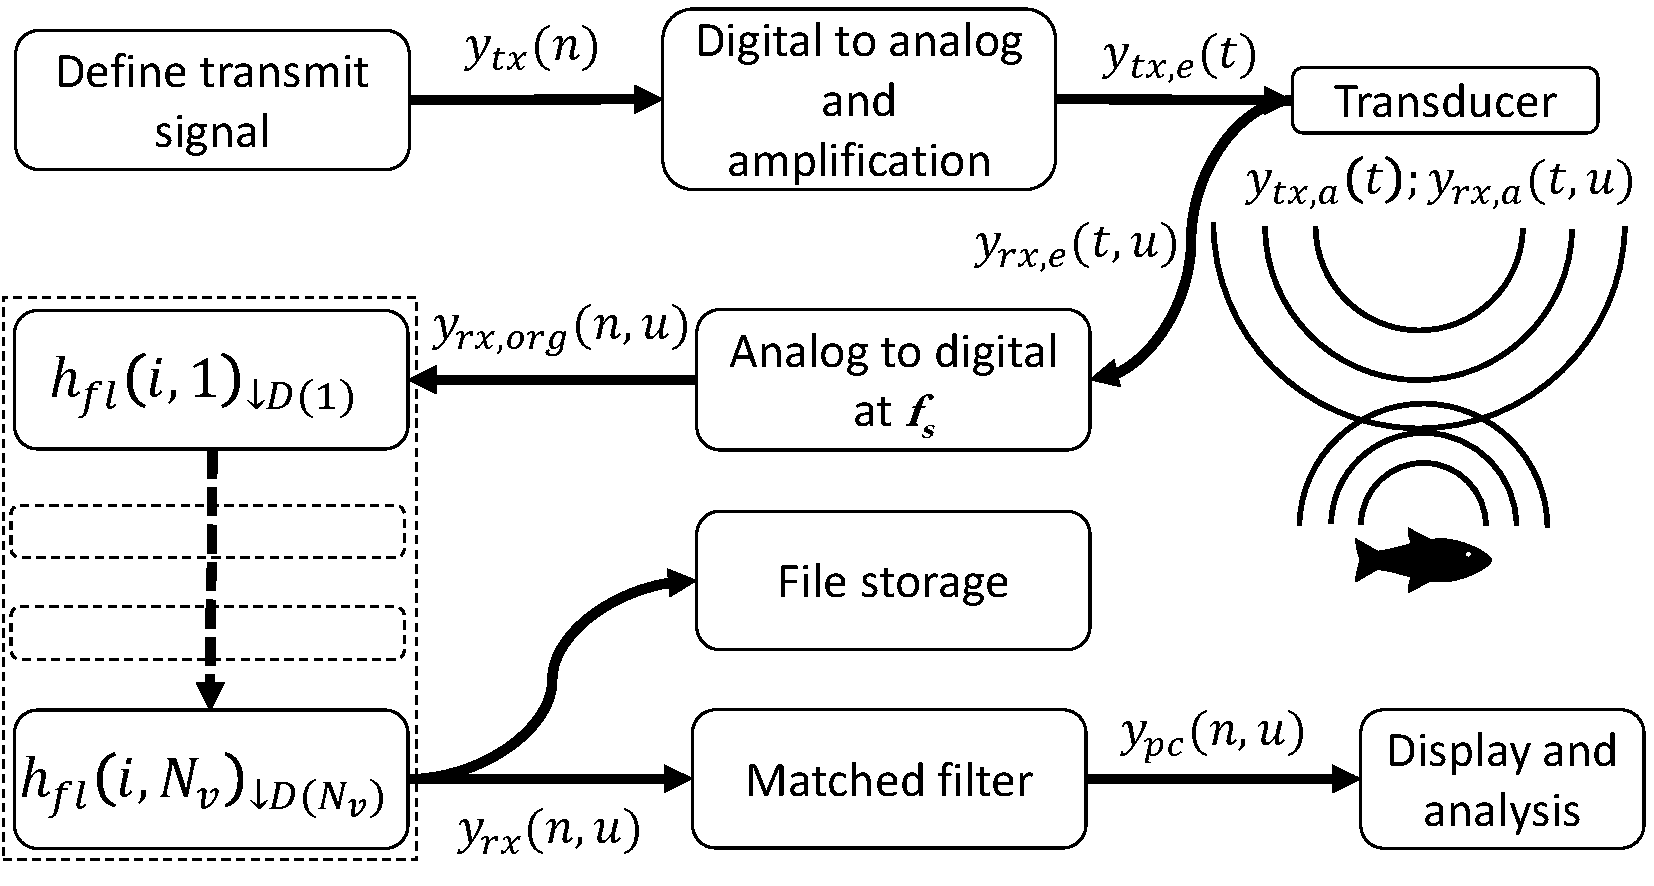
\includegraphics[width=16cm]{Fig_ek_sys}
\caption{\label{fi:ek_sys}Signal and data flow in the \ek{} system. An echosounder ping starts with the definition of a transmit signal (upper left) and ends with file storage (lower middle) and display and analysis (lower right).}
\end{figure}

\subsection{Signal generation}

The controlling computer program generates a short-duration digital transmit signal (a ping), $\ytx(\samplesymt)$, where $\samplesymt$ is the sample index in the discrete time domain. Typical broadband pulses are linear upsweep pulses windowed by an envelope function. The generated signal is converted to an analogue electric signal $\ytxe(\timesym)$ and amplified by the transceiver to obtain the analogue signal $\ytxe(\timesym)$, where $\timesym$ is the time for the signal. The analogue and amplified signals are passed on to the transducer to generate the transmitted acoustic signal $\ytxa(\timesym)$ in the water. For a splitbeam echosounder system, there are typically three or four channels to allow estimation of the angle of arriving echoes, and the signal is typically transmitted with equal power across the channels.

In the example a linear sweep enveloped by a Hanning window is implemented (Fig.~\ref{fi:ytx}), where the parameters are the initial frequency, the final frequency, the pulse duration, the sampling rate, and the proportion of the signal that is tapered in each end, respectively. A slope of 0 and .5 indicates no tapering and tapering across the whole signal, respectively.
\begin{figure}
\includegraphics[width=16cm]{Fig_ytx}
\caption{\label{fi:ytx} Envelope of linear chirp pulses from 92 kHz to 158 kHz with a slope of 0.057 (blue) and 0.5 (orange).}
\end{figure}

\subsection{Signal reception}

The returning acoustic signal, $\yrxa(\timesym)$, is received by each transducer sector, $\channelsym$, and converted to an analog electric signal, $\yrxe(\timesym,\channelsym)$, in the transducer and received by corresponding receiver channels, $\channelsym$, in the transceiver. The received electric signal, $\yrxe(\timesym,\channelsym)$, from each channel, $\channelsym$, is pre-amplified, filtered by an analog anti-aliasing filter, and digitized in the transceiver at a frequency of $\fs$, creating the digital signal, $\yrxorg(\samplesymt,\channelsym)$.

To remove noise and reduce the quantity of data, the sampled signal from each channel is filtered and decimated in multiple stages, $\stagesym$, using complex bandpass filters, $\hfl(\genidxsym,\stagesym)$, and decimation factors, $\decfac(\stagesym)$. The individual filter coefficients for each filter and decimation stage are indexed by $\genidxsym$. The output signal from each channel, $\channelsym$, from each filter and decimation stage, $\stagesym$, is then given by:
%
\begin{equation}
\label{eq:yrx}
\yrx(\samplesymt,\channelsym,\stagesym) = \left( \yrx(\samplesymt,\channelsym,\stagesym-1) * \hfl(\genidxsym,\stagesym) \right)_{\downarrow \decfac(\stagesym)}, 
\stagesym = 1,\ldots,\nstages,
\end{equation}
%
where $\yrx(\samplesymt,\channelsym,0)$ is set to $\yrxorg(\samplesymt,\channelsym)$, being the signal before decimation, $*$ indicates convolution, $\downarrow$ indicates decimation by the factor $\decfac(\stagesym)$, and $\nstages$ is the total number of filter stages. The output signal from the final filter and decimation stage, $\yrx(\samplesymt,\channelsym,\nstages)$, is shortened to $\yrx(\samplesymt,\channelsym)$ for convenience. For the output signal, $\yrx(\samplesymt,\channelsym)$, the decimated sampling rate, $\fsdec$, is given by:
%
\begin{equation}
\label{eq:fsdec}
\fsdec = \fs\prod_{\stagesym=1}^{\nstages} \frac{1}{\decfac(\stagesym)}.
\end{equation}
%
The characteristics of the bandpass filter and decimation factors are chosen with regard to the desired operating bandwidth, noise suppression levels, impulse response duration, and other common filter characteristics, with the aim of maintaining sufficient information in the data. In the example $N_v=2$. The frequency responses of the filters are shown in Figure~\ref{fi:fir} and the corresponding filter coefficients and decimation factors are given in the test data set.

\begin{figure}
\includegraphics[width=16cm]{Fig_fir}
\caption{\label{fi:fir} The frequency response (filter gain) of the filters in our test set. The blue and orange curve represents the filter response of the first and second filter. The horizontal green line indicates the frequency range of the transmit signal.}
\end{figure}

The original sample data $\yrxorg(\samplesymt,\channelsym)$ are not available in the EK80 data files. Instead, the filtered and decimated complex samples from each transducer channel $\yrx(\samplesymt,\channelsym)$ are stored in the data files. The data are recorded in computer data files for display and analysis by processing software. Additional information, such as that from position and motion sensors and system configuration data is also included in the files.

\subsection{Pulse compression}
To increase signal-to-noise ratio and resolution along the acoustic beam a matched filter may be applied to the raw data samples \citep{turin1960}. This technique is also known as pulse compression \citep{klauder1960}. One approach for a matched filter is to use a normalized version of the ideal transmit signal as the replicate signal, filtered and decimated using the same filters and decimation factors as applied in Eq. \ref{eq:yrx}. The normalized ideal transmit signal, $\ytxnorm(\samplesymt)$, is given by:
%
\begin{equation}
\label{eq:ytxnorm}
\ytxnorm(\samplesymt) = \frac{\ytx(\samplesymt)}{\textrm{max}(\ytx(\samplesymt))}\end{equation}
%
where $\textrm{max}$ is the maximum value of $\ytx(\samplesymt)$. The filtered and decimated output signal, $\ytxnorm(\samplesymt,\stagesym)$, from each filter stage, $\stagesym$, using the normalized ideal transmit signal, $\ytxnorm(\samplesymt)$, as the input signal, is given by:
%
\begin{equation}
\label{eq:FilterStagesTX}
\ytxnorm(\samplesymt,\stagesym) = \left[ \ytxnorm(\samplesymt,\stagesym-1) * \hfl(\genidxsym,\stagesym) \right]_{\downarrow \decfac(\stagesym)}, 
\stagesym = 1,\ldots,\nstages,
\end{equation}
%
where $\ytxnorm(\samplesymt,0)$ is set to $\ytxnorm(\samplesymt)$. The output signal from the final filter and decimation stage, $\ytxnorm(\samplesymt,\nstages)$, is used as the matched filter and is denoted as $\ymf(\samplesymt)$  (Fig.~\ref{fi:y_mf_n}).
%
\begin{figure}
\includegraphics[width=16cm]{Fig_y_mf_n}
\caption{\label{fi:y_mf_n} The absolute value of the filtered and decimated output signal, $\ymf(\samplesymt)$, that is used for the pulse compression.}
\end{figure}

The auto correlation function of the matched filter signal and the effective pulse duration, defined as the pulse duration at transmit power $\ptxe$ which produces the same energy as the actual transmitted pulse, will be used in later processing steps and are defined as
\begin{equation}
\label{eq:TXAuto}
\ymfauto(\samplesymt) = \frac{\ymf(\samplesymt)*\ymf^*(-\samplesymt)}{||\ymf||^2_2}
\end{equation}
and
\begin{equation}
\label{eq:TauEff}
\teff = \frac{\sum \ptxauto(\samplesymt)}{\textrm{max}(\ptxauto(\samplesymt))\fsdec},
\end{equation}
where
\begin{equation*}
%\label{eq:TauEff}
\ptxauto(\samplesymt)  =  |\ymfauto(\samplesymt)|^2
\end{equation*}
is the square of the absolute value of the matched filter autocorrelation function, and the summation is calculated over a duration of twice the nominal pulse duration, $2\tnom$.

\begin{figure}
\includegraphics{Fig_ACF}
\caption{The autocorrelation function $\ptxauto$ from the example. The corresponding $\teff=0.1$ ms and $\tnom=2$ ms\label{fi:ACF}.}
\end{figure}

To perform pulse compression the received signal, $\yrx(\samplesymt,\channelsym)$, is convolved with a complex conjugated and time-reversed version of the matched filter signal with the matched filter signal, and here also normalized with the $l^2$-norm of the matched filter to maintain received signal power. The pulse compressed signal, $\ypc(\samplesymt,\channelsym)$, then becomes
\begin{equation}
\label{eq:PulseComp}
\ypc(\samplesymt,\channelsym) = \frac{\yrx(\samplesymt,\channelsym)*\ymf^*(-\samplesymt)}{||\ymf||^2_2},
\end{equation}
%
where $||\ymf||$ indicates the $l^2$-norm of $\ymf$, also known as the Euclidean norm. The received power samples are then used to estimate target strength and volume backscattering strength. For estimating received power samples, the average signal, $\ypc(\samplesymt)$, over all transducer sectors, $\nchannels$, is used:
%
\begin{equation}
\label{eq:SumSig}
\ypc(\samplesymt) = \frac{1}{\nchannels} \sum_{\channelsym = 1}^{\nchannels} \ypc(\samplesymt,\channelsym).
\end{equation}
%
Compensation of echo strength for position in the acoustic beam requires an estimate of the echo arrival angle. This is obtained using the splitbeam method \citep{burdic1991}, which for broadband pules can be implemented with the angle values contained in the complex-valued $\ypc(\samplesymt)$ data, in combination with knowledge of transducer sector geometry. The principle is demonstrated with a transducer that is divided into four quadrants (Fig. \ref{fi:trd_quad}). In this example the summed signals from four halves (1+2, 2+3, 3+4, 4+1) are calculated as:
\begin{eqnarray}
\label{eq:SumHalves}
y_{\textrm{pc,fore}}(\samplesymt) & = & \frac{1}{2} \left( \ypc(\samplesymt,3)+\ypc(\samplesymt,4) \right),\\
y_{\textrm{pc,aft}}(\samplesymt) & = & \frac{1}{2} \left( \ypc(\samplesymt,1)+\ypc(\samplesymt,2) \right),\\
y_{\textrm{pc,star}}(\samplesymt) & = & \frac{1}{2} \left( \ypc(\samplesymt,1)+\ypc(\samplesymt,4) \right),\\
y_{\textrm{pc,port}}(\samplesymt) & = & \frac{1}{2} \left( \ypc(\samplesymt,2)+\ypc(\samplesymt,3) \right),
\end{eqnarray}
%
where fore, aft, star(board), and port indicate the relevant transducer halves.
\begin{figure}
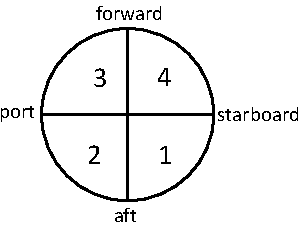
\includegraphics{Fig_trd_quad}
\caption{\label{fi:trd_quad}Transducer divided into four quadrants. The labels are directions often used when a transducer is mounted on a ship.}
\end{figure}
%


\subsection{Power and angle samples}
The transceiver measures voltage over a load, $\zrxe$, connected in series with the transducer impedance, $\ztde$. When calculating various acoustic properties, a system gain parameter will be used which assumes a matched receiver load. The total received power, $\prxe(\samplesymt)$, from all transducer sectors for a matched receiver load (Fig. \ref{fi:impedances}) is given by: 
\begin{equation}
\label{eq:prx}
\prxe(\samplesymt) = \nchannels\left( \frac{|\ypc(\samplesymt)|}{2\sqrt{2}} \right)^2 \left( \frac{|\zrxe+\ztde|}{\zrxe} \right)^2 \frac{1}{|\ztde|}.
\end{equation}
%
\begin{figure}
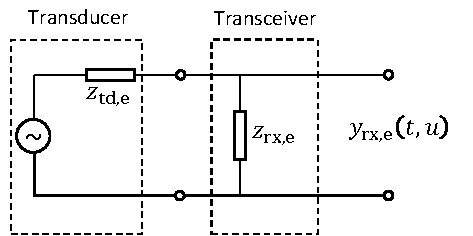
\includegraphics[width=16cm]{Fig_impedances}
\caption{\label{fi:impedances}Equivalent circuit diagram of transducer/transceiver with system impedances.}
\end{figure}

Forward/aft and port/starboard phase angles of target echoes are estimated by combining the transducer half signals thus: 
%
\begin{eqnarray}
\label{eq:phase1}
y_\along(\samplesymt) & = & y_{\textrm{pc,fore}}(\samplesymt) y_{\textrm{pc,aft}}^*(\samplesymt), \\
y_\athw(\samplesymt) & = & y_{\textrm{pc,star}}(\samplesymt) y_{\textrm{pc,port}}^*(\samplesymt),
\end{eqnarray}
%
where $y_\along(\samplesymt)$ is the electrical angle along the minor axis of the transducer (positive in the forward direction when ship-mounted) and $y_\athw(\samplesymt)$ the electrical angle along the major axis of the transducer (positive to starboard when ship-mounted), where complex signals are represented in the form $e^{j 2\pi \freqsym \timesym}$, where $j = \sqrt{-1}$. The physical echo arrival angles ($\along$ and $\athw$) are then given by:
%
\begin{eqnarray}
\label{eq:phase2}
\along(\samplesymt) & = & \arcsin\left( \frac{\atan\left( \Im(y_\along(\samplesymt)), \Re(y_\along(\samplesymt) \right)}{\anglefalong}\right) \\
\athw(\samplesymt) & = & \arcsin\left( \frac{\atan\left( \Im(y_\athw(\samplesymt)), \Re(y_\athw(\samplesymt) \right)}{\anglefathw}\right),
\end{eqnarray}
%
where $\anglefalong$ and $\anglefathw$ are constants that convert from phase angles to physical echo arrival angles (Fig.~\ref{fi:theta_phi}) and are derived from the transducer geometry and, $\fc$, the centre frequency of the chirp pulse \citep{ehrenberg1979}. The inverse sine is indicated by $\arcsin$,the four quadrant inverse tangent which returns values in the interval $[-\pi, \pi]$ inclusive is indicated by $\atan$, the real part of a complex number by $\Re$ and the imaginary part by $\Im$. As a mnemonic, the horizontal line in the symbol used for the forward/aft direction, $\along$, represents the pivot axis for the alongship angles and the near-vertical line in the $\athw$ symbol indicates the pivot axis for port/starboard angles.
%
\begin{figure}

\includegraphics[width=16cm]{Fig_theta_phi}
\caption{\label{fi:theta_phi}The physical angles $\along$ and $\athw$ for the target strength example data (see below). The single target can be seen around sample number 1000 where the angles are less variable.}
\end{figure}
\clearpage
\section{Target strength}

To illustrate calculation of target strength ($TS$) as a function of frequency, $TS(f)$, we use data collected on a 35 mm diameter tungsten carbide calibration sphere (WC35) suspended approximately 6 m below a 120 kHz transducer (Fig.~\ref{Fig_TS_echogram}). 

\begin{figure}
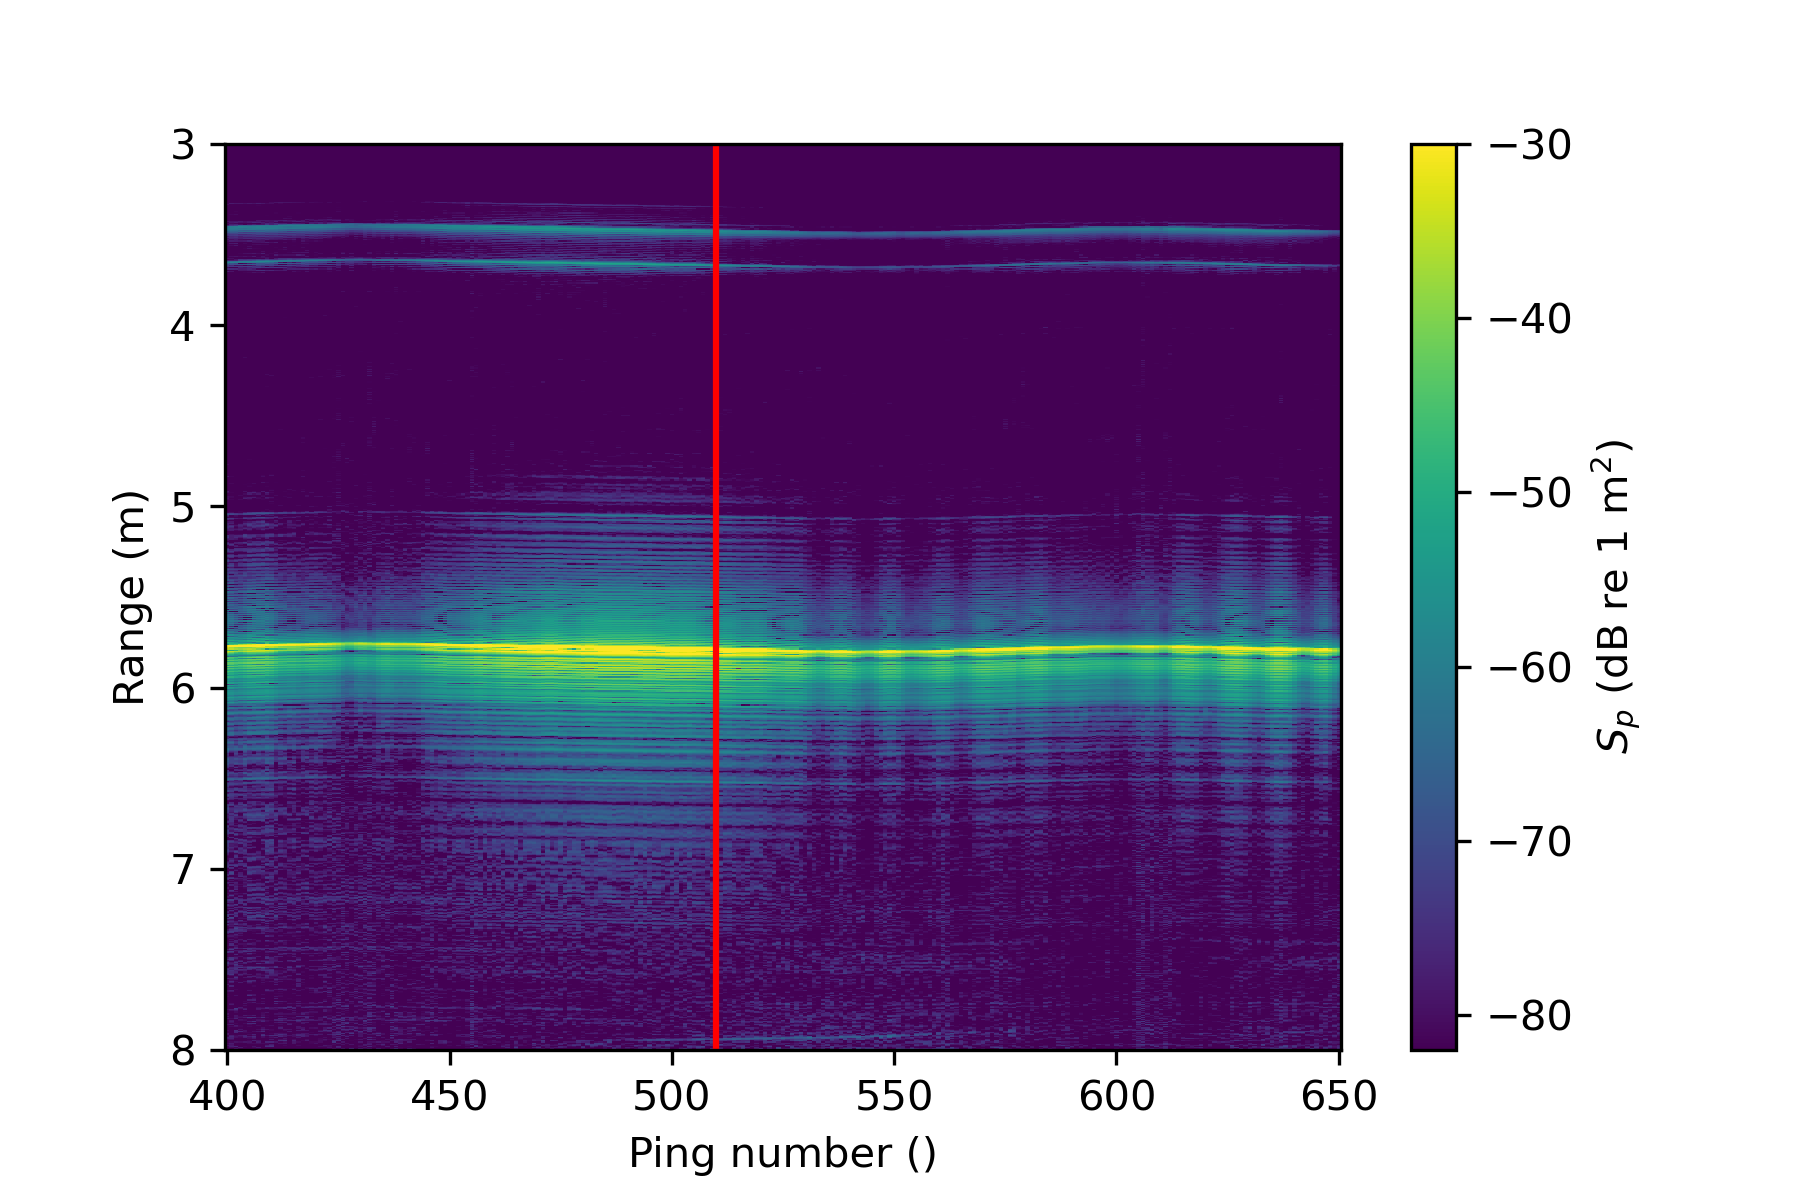
\includegraphics[width=16cm]{Fig_TS_echogram}
\caption{\label{Fig_TS_echogram} $\mysp$ as a function of ping number and range for a calibration sphere. The sphere is located at approximately 6 m range. The red vertical line indicates the ping that is used for illustrating the $\ts(\freqsym)$ processing.}
\end{figure}

Echoes from single targets are often characterised by their $\ts$, which is related to the differential backscattering cross section, $\bs$, via
%
\begin{equation}
\label{eq:TS_bs}
\ts = 10\log_{10}\left(\frac{\bs}{\rangeref^2}\right),
\end{equation}
%
where $\log_{10}$ is the logarithm with base 10 and $\rangeref$ is 1 m.

Generalizing the power-budget equation (i.e., sonar equation) for broadband signals \citep{lunde2016} yields, in logarithmic form, $TS$ at frequency $\freqsym$:
%
\begin{equation}
\label{eq:TS}
\ts(\freqsym) = 10\log_{10}(\prxetf(\freqsym)) + 40\log_{10}(\range) + 2\absorp(\freqsym) \range 
- 10\log_{10}\left( \frac{\ptxe \wlen^2(\freqsym) \gain^2(\along_t,\athw_t,\freqsym)}{16\pi^2} \right),
\end{equation}
%
where $\prxetf(\freqsym)$ is the Fourier transform of the received electric power in a matched load for a signal from a single target at frequency $\freqsym$, $\range_t$ is the range to the target, $\absorp(\freqsym)$ the acoustic absorption coefficient, $\ptxe$ the transmitted electric power, $\wlen$ the acoustic wavelength, and $\gain(\along,\athw,\freqsym)$ the transducer gain incorporating both the on axis gain $\gain_0(\freqsym)=\gain(0,0,\freqsym)$ and the beam pattern based on the estimated target bearing $(\along_t,\athw_t)$.

The point scattering strength, $\mysp(\samplesymt)$, is estimated by applying Eq. \ref{eq:TS} to the received digitized power samples using the on-axis gain value and $f$ set to the centre frequency of the broadband pulse, $\fc$: 
\begin{equation}
\label{eq:Sp}
\mysp(\samplesymt) = 10\log_{10}(\prxe(\samplesymt)) + 40\log_{10}(\range(\samplesymt)) 
+ 2\absorp(\fc) \range(\samplesymt) - 10\log_{10}\left( \frac{\ptxe \wlen^2(\fc) \gainzero^2(\fc)}{16\pi^2} \right),
\end{equation}
%
noting that $\mysp(\samplesymt)$ is an average over frequency of all echoes from single or multiple targets received at sample $\samplesymt$.

Based on the point scattering strength samples and the phase angle samples, single targets can be detected, and range and bearing to the single targets can be estimated. This is typically achieved through a single echo detection algorithm (SED). Here we will assume that the samples from the pulse compressed data $\ypc(\samplesymt)$ originating from single target already have been identified, noting that the number of samples after the detected target may be higher than those those before the peak to include scattering processes that occur in actual targets (as opposed to ideal point targets). The alongship angle $\along(\samplesymt)$, athwartship angle $\athw(\samplesymt)$ and sample number $n$ at the \emph{peak} power $\prxe(\samplesymt)$ within the detected target are used as estimates for $\along_t$, $\athw_t$ and $r_t$, respectively (Fig. \ref{fi:theta_phi}). A simple pseudo SED algorithm is implemented in the code for illustrative purposes.

From the autocorrelation function of the matched filter signal, $\ymfauto(\samplesymt)$, the equivalent number of samples around the peak are extracted to create the reduced autocorrelation signal of the matched filter signal, $\ymfautored(\samplesymt)$ (Fig.~\ref{fi:SED}). Depending on the target scattering characteristics and the distance to any adjacent single targets, the number of samples around the peak echo level in $\ypctarget(\samplesymt)$ that contain the majority of the echo energy can be more or less than the total number of samples around the peak of $\ymfauto(\samplesymt)$. If the number of samples around the target is more than the total number of samples around the peak of $\ymfauto(\samplesymt)$ all samples around the peak of $\ymfauto(\samplesymt)$ are used. If the number of samples around the target is less than the total number of samples around the peak of $\ymfauto(\samplesymt)$, this lower number is used to create $\ymfautored(\samplesymt)$.
%
\begin{figure}
\includegraphics[width=16cm]{Fig_singleTarget}
\caption{\label{fi:SED} The $\prxe(\samplesymt)$ power (upper) and split beam angles ($\along_t$ and $\athw_t$) (middle) for the single target. The orange vertical line corresponds to the range $r_t$ for the single target. The $\ymfautored(\samplesymt)$ (lower) is the autocorrelation function of the transmit signal reduced to the length of the target signal and aligned with the peak power of the target.}
\end{figure}

The discrete Fourier transforms of the target signal, $\ypctargetf(\samplesymf)$, and the reduced auto correlation signal, $\ymfautoredf(\samplesymf)$, are given by:
\begin{eqnarray}
\label{eq:DFT_Target_Auto}
\ypctargetf(\samplesymf) & = & \dft_\ndft(\ypctarget(\samplesymt)),\\
\ymfautoredf(\samplesymf) & = & \dft_\ndft(\ymfautored(\samplesymt)),
\end{eqnarray}
where $\dft$ indicates the Fourier transform of length $\ndft$ and $\samplesymf$ the sample index in the frequency domain.
The nomalized discrete Fourier transform of the target signal, $\ypctargetnormf(\samplesymf)$, (Fig. \ref{fi:TS}) is then calculated by: 
%
\begin{equation}
\label{eq:DFT_Target_Auto_Norm}
\ypctargetnormf(\samplesymf) = \frac{\ypctargetf(\samplesymf)} {\ymfautoredf(\samplesymf)}.
\end{equation}

Assuming, as a first approximation, that the impedances of the transceiver and transducer are independent of frequency, the received power into a matched load, $\prxetf(\samplesymf)$, is then estimated by:
\begin{equation}
\label{eq:prx_FFT_target}
\prxetf(\samplesymf) = \nchannels\left( \frac{|\ypctargetnormf(\samplesymf)|}{2\sqrt{2}} \right)^2 
\left( \frac{|\zrxe+\ztde|}{|\zrxe|}\right)^2 \frac{1}{|\ztde|}, % All channels (*4), matched load (/2), and effective values (/sqrt(2))
\end{equation}
%
noting that any variation of impedance with frequency will be reflected in the $\gainzero$ obtained from the calibration process.

Target strength can then be estimated using Eq. \ref{eq:TS}:
\begin{equation}
\label{eq:TS_f}
\ts(\freqsym) = 10\log_{10}(\prxetf(\samplesymf)) + 40\log_{10}(\range_t) + 2\absorp(\freqsym)\range_t - 10\log_{10}\left( \frac{\ptxe \wlen^2 \gain^2(\along_t,\athw_t,f)}{16\pi^2} \right)
\end{equation}
where the sample index $\samplesymf$ corresponding to frequency $\freqsym$ can be estimated using
\begin{equation}
\label{eq:m(f)}
\samplesymf = \lfloor \frac{\freqsym}{\fsdec} \ndft \rfloor \mod \ndft
\end{equation}
%
\begin{figure}
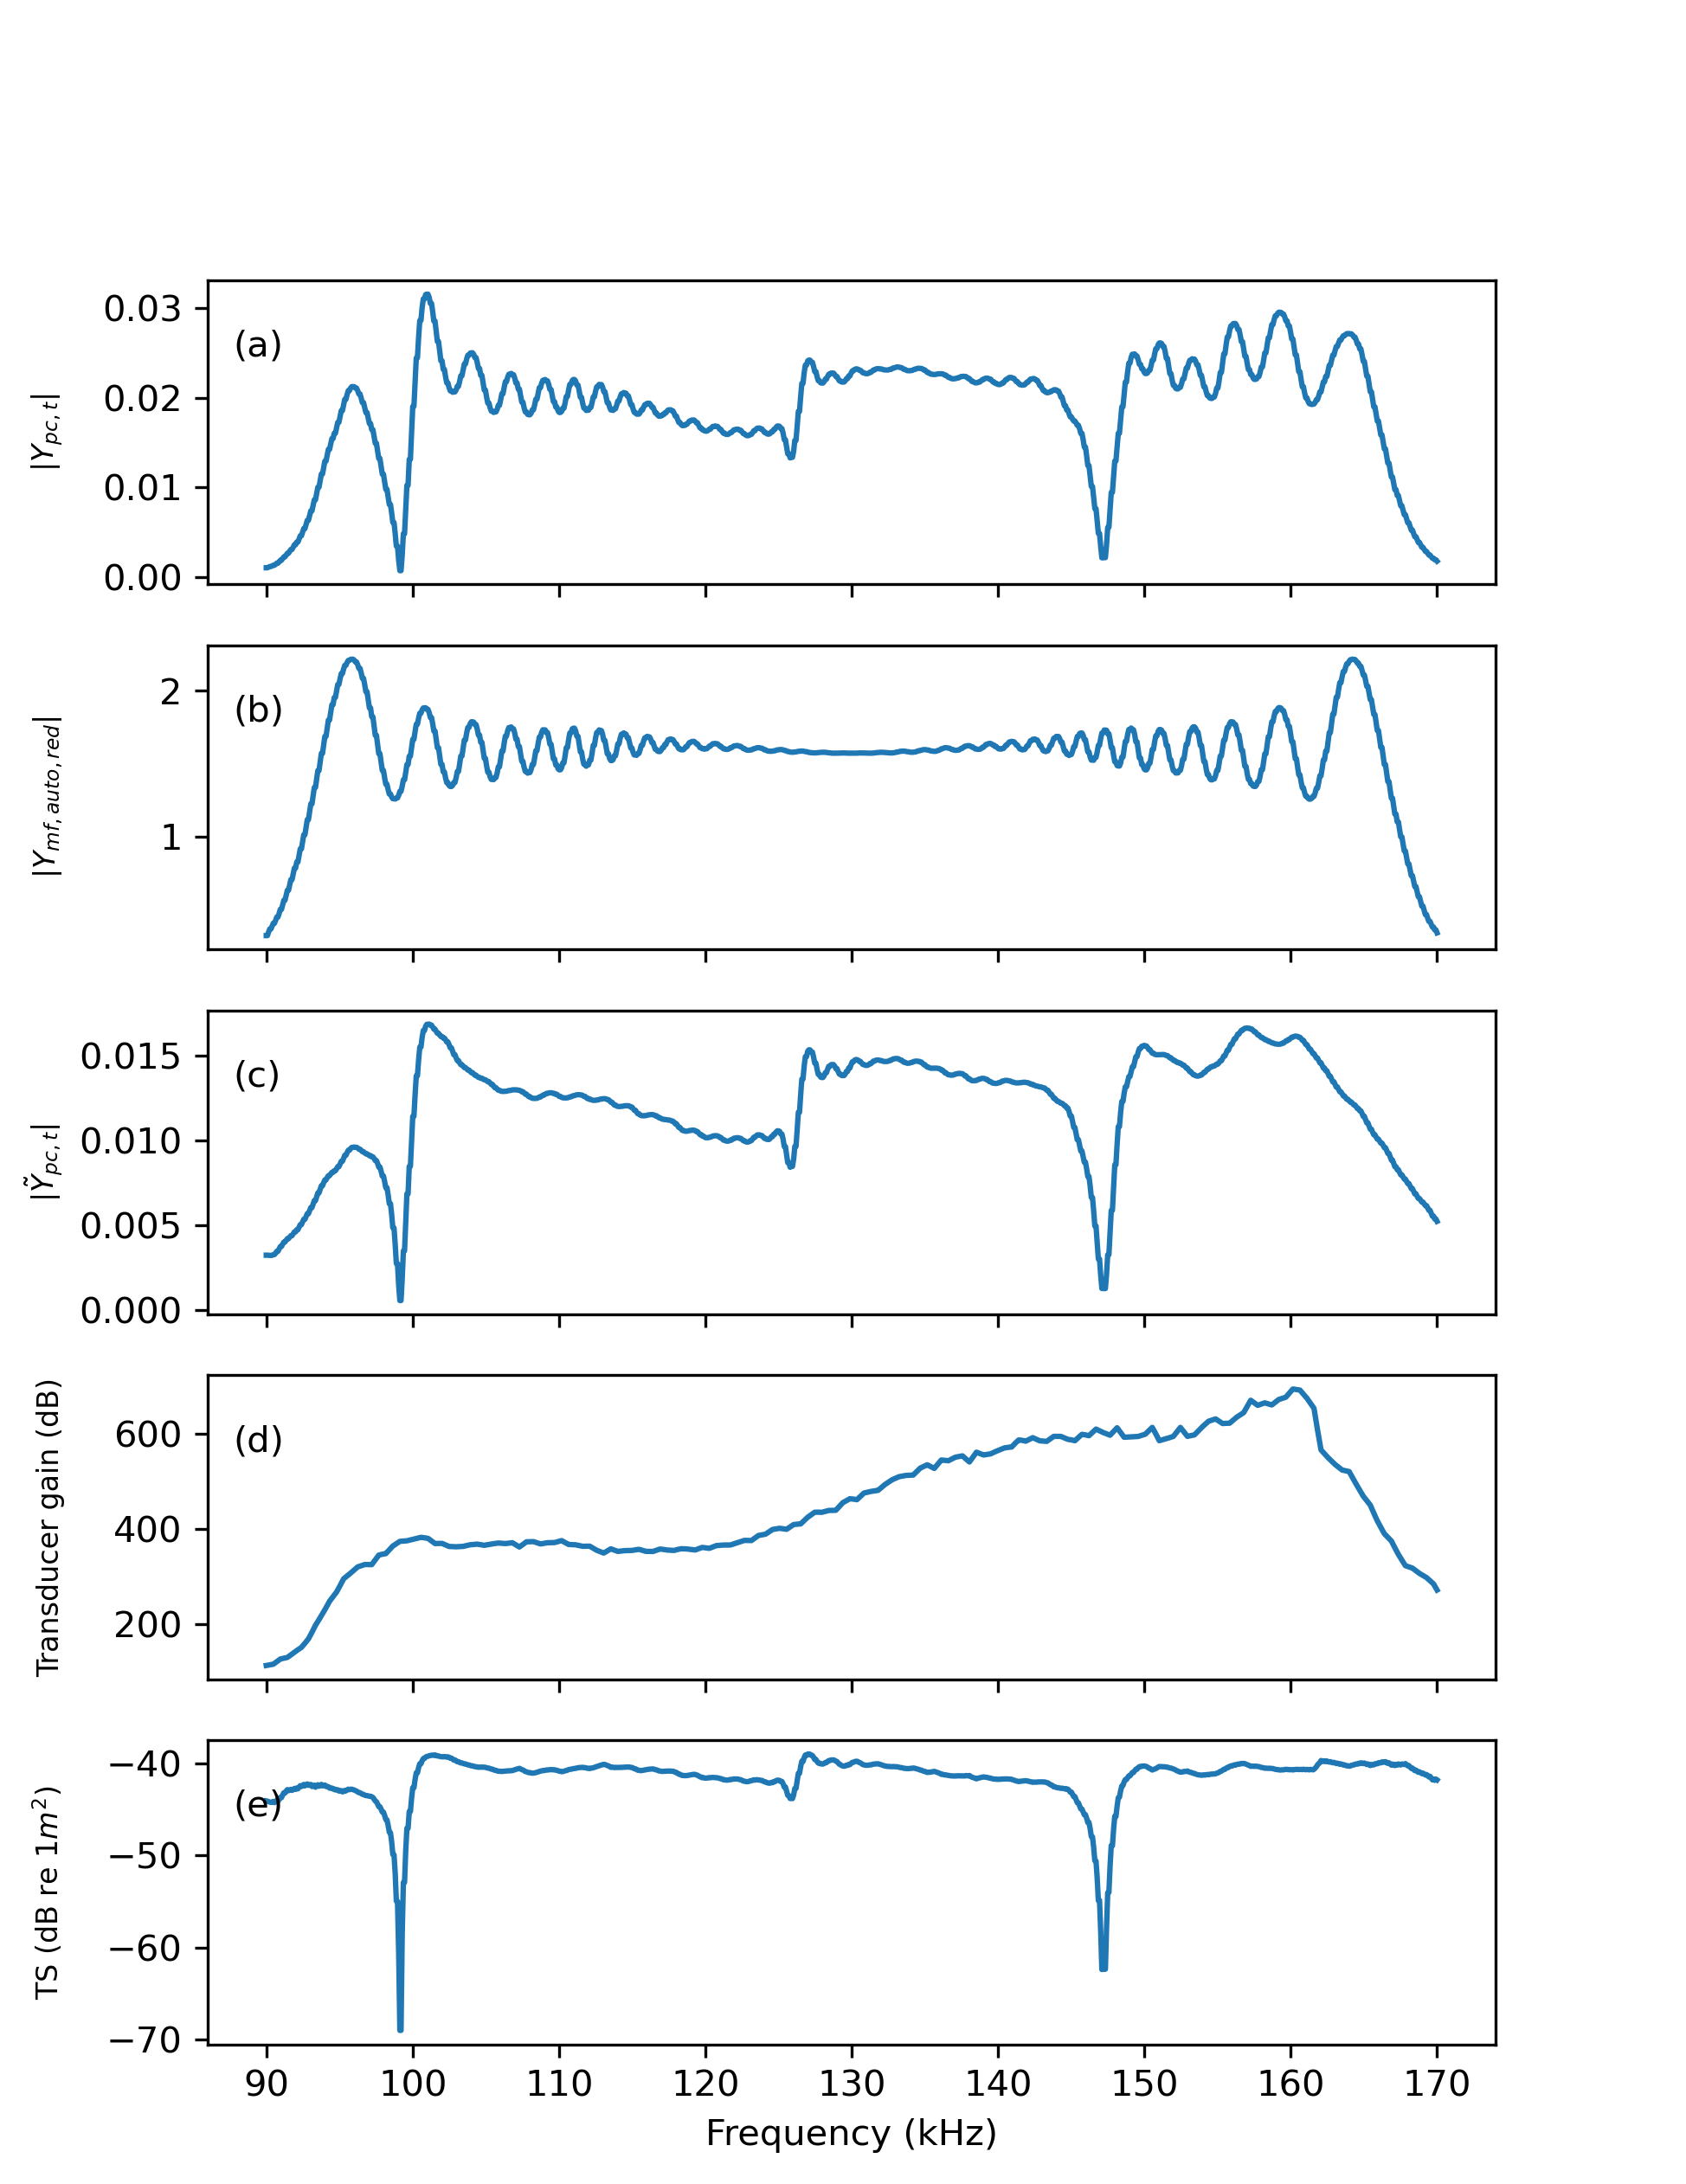
\includegraphics[width=16cm]{Fig_TS}
\caption{\label{fi:TS}The discrete Fourier transform of the target signal $\ypctargetf(\samplesymf)$ (a) and the reduced auto correlation signal $\ymfautoredf(\samplesymf)$ (b), the normalized discrete Fourier transform of the target signal $\ypctargetnormf(\samplesymf)$ (c), transducer gain $(10\log_{10}\gain^2(\along_t,\athw_t,\freqsym))$ (d), and the estimated TS(f) (e).}
\end{figure}
%
A frequency modulated pulse scattered by a metallic sphere will exhibit frequencies at which very little energy is returned due to destructive interference \citep{stanton2008}. This is visible in the $\ts$ (Fig. \ref{fi:TS}) and agrees well with theoretical estimates of the backscatter from spheres \citep{maclennan1981}.

\section{Volume backscattering strength}

To illustrate calculation of volume backscattering strength as a function of frequency,  $\sv(f)$, we use data collected from a school of non-swimbladdered fish (Fig.~\ref{Fig_Sv_echogram}) collected with a 120 kHz centre frequency transducer. 

Echoes from multiple scatterers can be quantified using volume backscattering strength, $\sv$, being the density of backscattering cross sections, and is given by:
%
\begin{equation}
\label{eq:sv}
\sv  =  10\log_{10}\frac{\sum\bs}{V}.
\end{equation}
%
where $V$ is the volume occupied by the scattering targets. The power-budget equation for multiple targets is then:
%
\begin{equation}
\label{eq:sv_f}
\sv(\freqsym) = 10\log_{10}(\prxevf(\freqsym)) + 20\log_{10}(\range_c) + 2\absorp(\freqsym)\range_c 
- 10\log_{10}\left( \frac{\ptxe \wlen^2 \cw \tslide \eqang(\freqsym) \gainzero^2(\freqsym)}{32\pi^2} \right), 
\end{equation}
%
where $\prxevf(\freqsym)$ is the received electric power in a matched load for the signal from a volume at frequency $\freqsym$, $\cw$ the sound speed, $\tslide$ the duration of the time window, excluding the zero-padded portion if applied, used for evaluating the frequency spectrum, $\range_c$ is the range to the centre of the range volume covered by $\tslide$, and $\eqang(\freqsym)$ is the two-way equivalent beam angle. The two-way equivalent beam angle is a function of frequency that is derived from an empirical estimate of $\eqang$ at the nominal frequency, $\fn$:
\begin{equation}
\label{eq:PsiFc}
\eqang(f) = \eqang(\fn)\left(\frac{\fn}{f}\right)^2.
\end{equation}

\begin{figure}
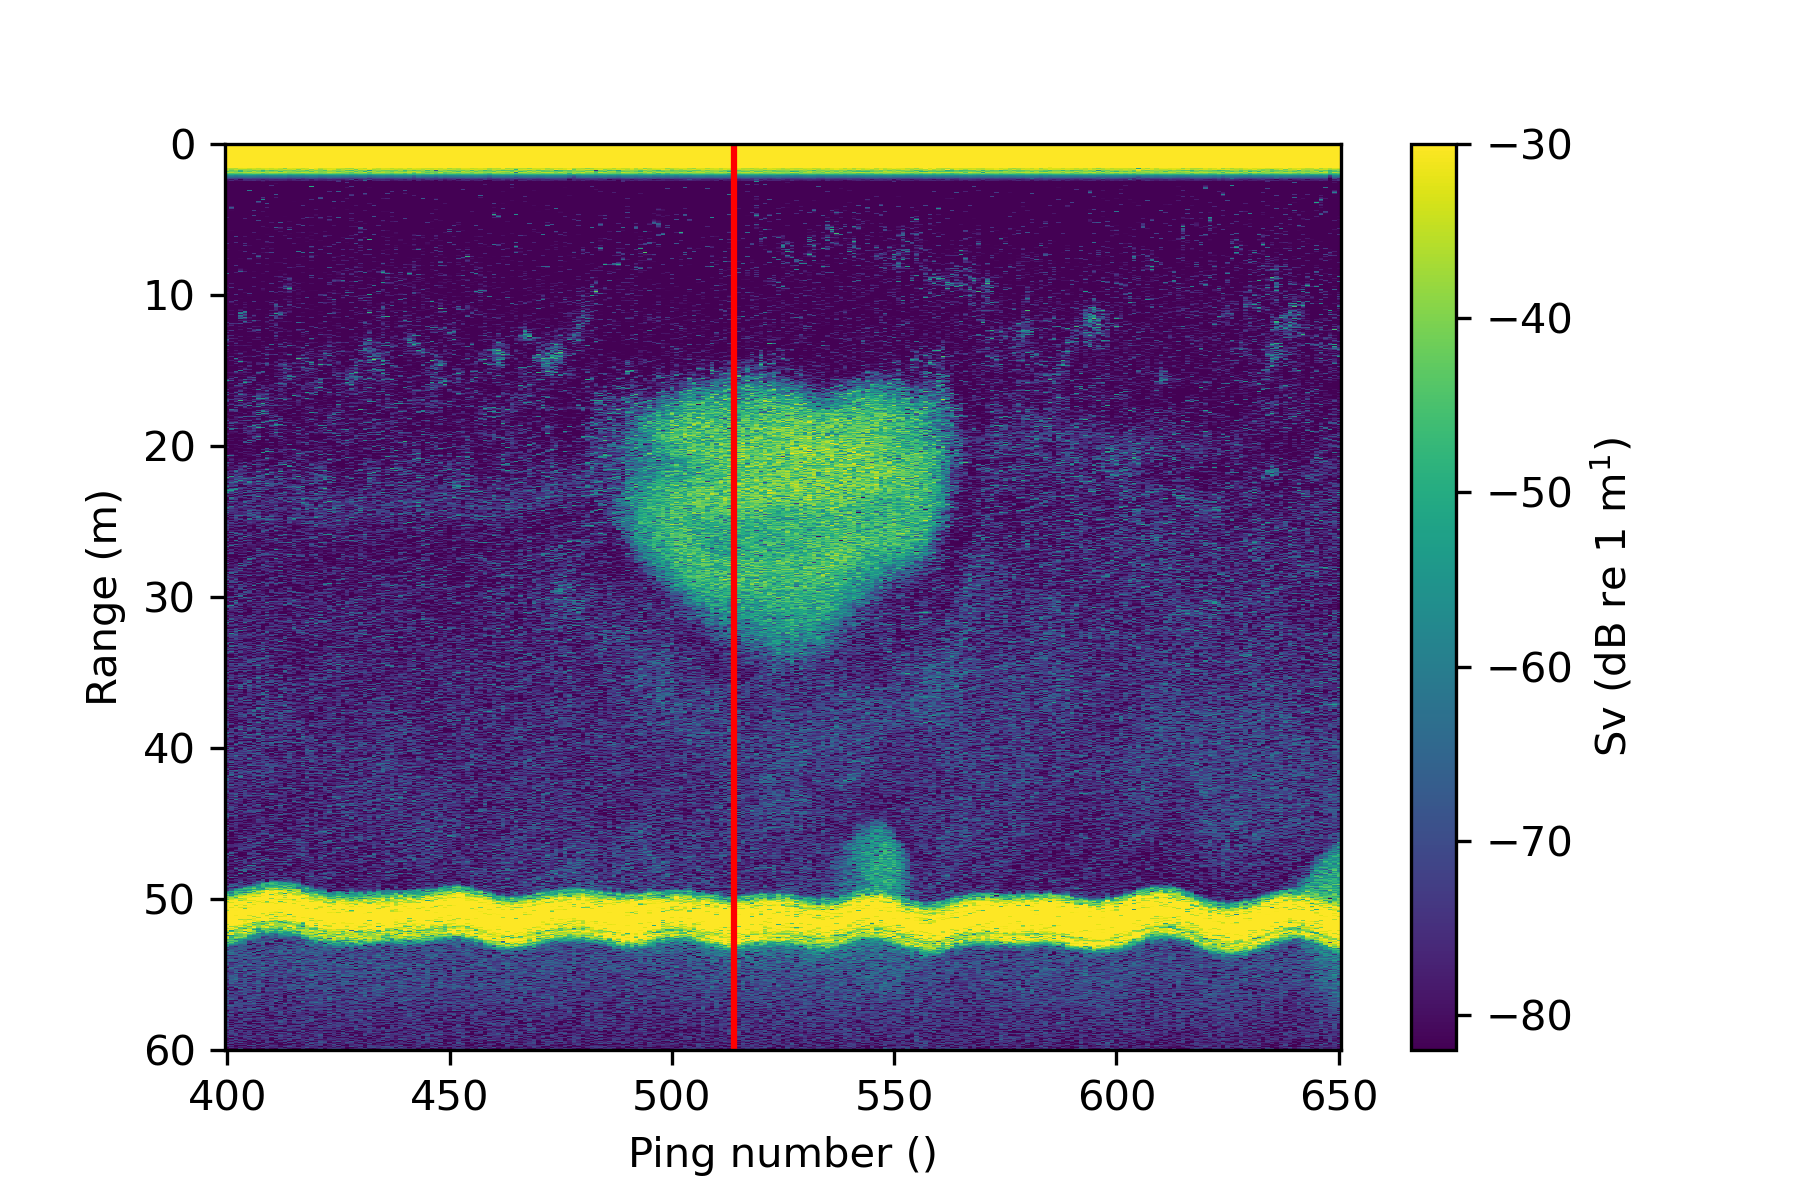
\includegraphics[width=16cm]{Fig_Sv_echogram}
\caption{\label{Fig_Sv_echogram} Sv as a function of ping number and range range ($\samplesymt$) for the raw data file used in the Sv(f) example. The upper yellow area shows the transmit pulse, a fish school is seen as a registration between 15 and 35 m range, and the sea floor is seen at approximately 50 m. The red vertical line indicates the ping that is used for illustrating the $\sv(\freqsym)$ processing.}
\end{figure}

Volume backscattering samples compressed over the operational frequency band are estimated by applying Eq. \ref{eq:sv_f} to the received digitized power samples using the on-axis gain value with $f$ set to the centre frequency of the broadband pulse, $\fc$:
\begin{equation}
\label{eq:Sv}
\begin{split}
\sv(\samplesymt)  =  10\log_{10}(\prxe(\samplesymt)) + 20\log_{10}(\range_c(\samplesymt)) + 2\absorp(\fc)\range_c(\samplesymt) \\
- 10\log_{10}\left( \frac{\ptxe \wlen^2(\fc) \cw \teff \eqang(\fc) \gainzero^2(\fc)}{32\pi^2} \right).
\end{split}
\end{equation}
%noting that $\sv(\samplesymt)$ is an average over frequency of all echoes received at sample $\samplesymt$. In this case, the time window, $\tslide$, is the effective pulse duration, $\teff$, resulting from pulse compression.

Compensation of spherical spreading loss requires compensation of received power by a factor of $r_c^2$, and hence compensation of amplitude by a factor of $\range_c$:
%
\begin{equation}
\label{eq:spreadcomp}
\ypcspread(\samplesymt) = \ypc(\samplesymt)\range_c(\samplesymt).
\end{equation}
%
where $\ypcspread(\samplesymt)$ is the pulse compressed signal compensated for spherical spreading. A discrete Fourier transform is performed on the range compensated pulse compressed sample data using a normalized sliding Hanning window, $\hannw(\genidxsym)$. The duration, $\tslide$, of the sliding window is chosen as a compromise between along-beam range resolution and frequency resolution. We suggest that it be at least twice the pulse duration and for computational efficiency reasons should result in a number of samples, $\nw$, which is a power of 2.

The normalised Hanning window, $\hannwnorm$, is given by: 
%
\begin{equation}
\label{eq:hannw}
\hannwnorm(\genidxsym) = \frac{\hannw(\genidxsym)}{\left( \frac{||\hannw||_2}{\sqrt{\nw}} \right)}, i = \frac{-\nw}{2}, \ldots, \frac{\nw}{2}
\end{equation}
%
and the discrete Fourier transform of the windowed data, $\ypcvolumef(\samplesymf)$, is then obtained from:
%
\begin{equation}
\label{eq:FFT_volume}
\ypcvolumef(\samplesymf) = \dft_\ndft 
\left( \hannwnorm(\genidxsym) \left(\ypcspread (\genidxsym+\samplesymt) \left[ u(\genidxsym + \frac{\nw}{2}) - u(\genidxsym - \frac{\nw}{2}) \right] \right) \right),
\end{equation}
%
where $u(\genidxsym)$ is the step function and $\samplesymt$ is the sample data index for the centre of the sliding window. The discrete Fourier transform of the auto correlation function of the matched filter signal, $\ymfautof(\samplesymf)$, also needs to be evaluated at the same frequencies:
%
\begin{equation}
\label{eq:FFT_TX_Auto}
\ymfautof(\samplesymf)  =  \dft_\ndft (\ymfauto(\samplesymt)).
\end{equation}

The normalized discrete Fourier transform of the windowed data, $\ypcvolumenormf(\samplesymf)$, is then given by:
%
\begin{equation}
\label{eq:FFT_volume_norm}
\ypcvolumenormf(\samplesymf) = \frac{\ypcvolumef(\samplesymf)}{\ymfautof(\samplesymf)},
\end{equation}
%
and received power into a matched load, $\prxevf(\samplesymf)$, is estimated from:
%
\begin{equation}
\label{eq:prx_FFT_volume}
\prxevf(\samplesymf) = \nchannels \left( \frac{|\ypcvolumenormf(\samplesymf)|}{2\sqrt{2}} \right)^2 \left( \frac{|\zrxe+\ztde|}{|\zrxe|}\right)^2 \\
\frac{1}{|\ztde|}. % All channels (*4), matched load (/2), and effective values (/sqrt(2))
\end{equation}
%
Finally, the discretized estimate of $\sv(\freqsym)$, $\sv(\samplesymf)$, is given by:
%
\begin{equation}
\label{eq:Sv_FFT}
\sv(\freqsym) = 10\log_{10}(\prxevf(\samplesymf)) + 2\absorp(\freqsym) \range_c - 10\log_{10}\left( \frac{\ptxe \wlen^2 \cw \tslide \eqang(\freqsym) \gainzero^2(\freqsym) }{32\pi^2} \right).
\end{equation}
where the sample index $\samplesymf$ corresponding to frequency $\freqsym$ can be estimated using Eq. {\ref{eq:m(f)}}.

By selecting a set of centre samples $\timesym$, $\sv$ values can be presented as a function of range ($\samplesymt$) and frequency ($\freqsym$) for each ping. The range for centre samples $\samplesymt$ could be chosen as half the window length or any other grid that the user prefer the data presented to be in. This can be useful when combining the $\sv(\freqsym)$ across a range of transducers. In our example we have simply chosen the set of centre samples as the original range samples (Fig.~\ref{Fig_Sv_m_n}).

\begin{figure}
\includegraphics[width=16cm]{Fig_Sv_m_n}
\caption{\label{Fig_Sv_m_n} $\sv$ as a function of frequency ($\samplesymf$) and range ($\samplesymt$) for a single ping.}
\end{figure}

For acoustic abundance estimation and classification purposes it is common to integrate $\sv$ over a range (15 to 34 m in the example, covering a school of non-swimbladdered fish, Fig.~\ref{Fig_Sv_echogram}). It is normal to average $\sv$ over several pings to obtain an unbiased estimate, but here just one ping is used for illustrative purposes (Fig.~\ref{Fig_Sv_avg}). Even though this is for a single ping it is still possible to observe a positive slope of the frequency response that is indicative of non-swimbladdered fish. 

\begin{figure}
\includegraphics[width=16cm]{Fig_Sv_avg}
\caption{\label{Fig_Sv_avg} $\sv$ as a function of frequency averaged over a depth interval covering a fish school.}
\end{figure}

The trend for increasing $\sv$ with frequency is well-known for non-swimbladderred fish \citep{korneliussen2010} and is consistent with the trend observed in this example. In contrast to data from isolated scatterers, such as metallic spheres, the benefit of pulse compression on the backscatter from an object that generates many overlapping echoes is not immediately obvious (Fig.~\ref{Fig_Sv_echogram}).

\section{Discussion}

The use of broadband signals in fisheries acoustics is a developing field, and our contribution represents a comprehensive description of data processing steps. The inclusion of corresponding computer code ensures a more complete description. One could also envision that signal processing steps designed for specific purposes beyond these standard parameters can be developed, and our code can serve as a starting point for this. We also envision that the paper and code be used both for educational purposes and for understanding the standard broadband signal processing.

The contribution includes all the minor details required for the processing steps to work in practice. This includes steps well founded in the literature as well as practical and more ad-hoc choices. Handling of gaps in the calibration data, the choice of transmit pulse including tapering, calculation of efficient pulse duration, and decimation factors and filtering. When convolving the received signal with the transmit pulse, there are various approaches to handle edge cases and in our implementation we chose to exclude the edge cases. We have also assumed a four-sector transducer, and the code must be adapted to other beam configurations if other configurations are needed. When estimating $\ts(\freqsym)$ and $\sv(\freqsym)$ the resolution and accuracy will depend on the length, $\ndft$, of the Fourier transform and the actual choice will be a compromise between accuracy and computational speed. Our objective is not to provide an evaluation of all these choices, but to serve as a startin point.

$\ts(\freqsym)$ is a common metric for studying single targets, used to extract features for single individuals. Features includes size, target classification and, behaviour through tracking. In our implementation, calculation of $\ts(\freqsym)$ assumes that a single target has successfully been identified. This requires a robust single target detector. Several SED algorithms exist and differing such algorithms may be required depending on the situation. Typical SED algorithms are based on traditional single frequency pulses and by utilizing the additional information in broadband echoes improved SEDs may be envisioned, but this is outside the scope of this paper.

$\sv(\freqsym)$ is a key parameter for echo integration. To estimate $\sv(\freqsym)$ a Fourier transform is used, repeatedly applied via a sliding window in range. The chosen size of the window is two times the pulse length, and is chosen as a compromise between spatial and frequency resolution. Since the duration of the sliding window can cause the spreading loss compensation to differ between the beginning and end of the window, the compensation for spreading loss is performed on the pulse compressed time domain data before the transform. Absorption loss compensation is also range dependent (and frequency dependent), but is insignificant for typical marine ecosystem echosounder operating frequencies between the beginning and the end of the window for relatively short range windows. The compensation for absorption loss is therefore performed after applying the discrete Fourier transform. The choice of window also allows the data to be split onto a predefined range-frequency grid, which can then be used to fit data across transducers to an n-dimensional tensor typically employed by deep learning methods \citep[e.g.]{brautaset_acoustic_2020}.

The formulation presented in this paper requires several frequency dependent parameters, such as transducer gain, two-way equivalent beam angle, and the water absorption coefficient, to quantitatively estimate $\ts(\freqsym)$ and $\sv(\freqsym)$. Methods to estimate these are not within the scope of this paper, but common practise is to use the conventional sphere backscatter calibration methodology \citep{demerCalibrationAcousticInstruments2015} slightly enhanced for broadband \citep{hobaekCharacterizationTargetSpheres2013,lavery2017}. We note that these methods do not provide an operational method to estimate $\teff$ or $\eqang(\freqsym)$, especially for ship-mounted transducers, and that empirical measurements of these parameters are necessary to fully calibrate both narrowband and broadband echosounders.

A set of equations and associated computer code for calculating calibrated, frequency-dependent, target strength and volume backscatter from broadband echosounder signals have been presented along with example code, providing a resource for those interested in learning and further developing broadband processing techniques. The processing equations and methodology presented in this paper are similar to those implements in version 1.12.4 and earlier of the \ek{} software.

\section{Conclusion}

A set of equations for calculating calibrated, frequency-dependent, target strength and volume backscatter from broadband echosounder signals have been presented along with example code, with reference to the \ek{} echosounder.

\section{Data Availability Statement}

The code and data associated with this article are available through GitHub through \url{https://github.com/CRIMAC-WP4-Machine-learning/CRIMAC-Raw-To-Svf-TSf}. The code and data for the pre-print is tagged version 0.9. The version for the printed paper is 1.0. Further developments will have higher version numbers.

\bibliography{Reference_database}

\end{document}
